\documentclass[final]{beamer}
\usepackage[orientation=portrait,size=a1,scale=1.18]{beamerposter}
\usepackage{lmodern}
\usepackage{graphicx}
\usepackage{booktabs}
\usepackage{amsmath,amssymb}
\usepackage{tikz}
\usepackage[T1]{fontenc}

% ---- cool teal palette (consistent with the CL reports) ----
\definecolor{theme}{HTML}{2b6a77}
\definecolor{themeD}{HTML}{1f4e58}
\definecolor{ink}{HTML}{232d33}
\definecolor{cardbg}{HTML}{f3f6f7}
\definecolor{ok}{HTML}{3f8161}
\definecolor{warn}{HTML}{b5651d}
\definecolor{muted}{HTML}{6b7a80}

\setbeamercolor{block title}{bg=theme,fg=white}
\setbeamercolor{block body}{bg=cardbg,fg=ink}
\setbeamertemplate{blocks}[rounded][shadow=false]
\setbeamertemplate{itemize items}[circle]
\setbeamercolor{itemize item}{fg=theme}
\setbeamercolor{itemize subitem}{fg=theme}
\setbeamerfont{block title}{size=\large,series=\bfseries}
\setbeamerfont{itemize/enumerate body}{size=\normalsize}

\newcommand{\pend}[1]{\textcolor{warn}{\textbf{#1}}}
\newcommand{\good}[1]{\textcolor{ok}{\textbf{#1}}}

% highlight box
\newenvironment{keybox}{%
  \begin{beamercolorbox}[sep=10pt,rounded=true,wd=\linewidth]{block body}%
  \begin{minipage}{0.94\linewidth}\color{themeD}}%
  {\end{minipage}\end{beamercolorbox}}

\begin{document}
\begin{frame}[t]

% ============ HEADER ============
\begin{center}
{\color{theme}\rule{\linewidth}{3pt}}\\[0.4ex]
{\veryHuge\bfseries\color{themeD} Detecting Sub-Millimetre Bone Fractures}\\[0.4ex]
{\Huge\bfseries\color{theme} via the X-ray Scatter-to-Primary Ratio}\\[0.6ex]
{\Large A Monte Carlo (OpenGATE\,10 / Geant4) Feasibility Study}\\[0.5ex]
{\large [Author Name]\quad$\bullet$\quad Baanwit Academy\quad$\bullet$\quad 2026 \quad$\bullet$\quad \textit{preliminary --- CL-3 \& CL-6 pending}}\\[0.3ex]
{\color{theme}\rule{\linewidth}{3pt}}
\end{center}
\vspace{0.4ex}

\begin{columns}[t]

% ================= LEFT COLUMN =================
\begin{column}{.475\textwidth}

\begin{block}{1. Introduction}
\begin{itemize}
  \item Hairline / sub-millimetre fractures are frequently \textbf{invisible on plain radiographs}: the attenuation contrast they create is tiny.
  \item \textbf{Hypothesis:} a fracture perturbs the local scatter field, leaving a signature in the \textbf{Scatter-to-Primary Ratio}
  \[ \mathrm{SPR}(x,y)=\frac{I_{\text{scatter}}}{I_{\text{primary}}} \]
  \item \textbf{Aim:} test by Monte Carlo whether this SPR signature is \emph{detectable}, \emph{statistically robust}, \emph{not an artifact}, and \emph{physically grounded}.
\end{itemize}
\end{block}

\begin{block}{2. Methods}
\begin{itemize}
  \item \textbf{Engine:} OpenGATE 10 (Geant4), Livermore physics; 80\,keV; compact bone (ICRU); AP pelvis; SPR map from primary/scatter separation at the detector.
  \item \textbf{Fracture models:} gap widths 0.306, 0.43, 0.54, 1.0\,mm.
  \item \textbf{Matched control (key):} the \emph{same} mesh with the gap filled $\Rightarrow$
  $\Delta\mathrm{SPR}=\mathrm{SPR}_{\text{frac}}-\mathrm{SPR}_{\text{ctrl}}$ isolates \textbf{only the fracture} (removes the mesh-tessellation confound).
  \item \textbf{Multi-seed significance:} $N{=}8$ independent seeds, common random numbers; \emph{a-priori} ROI $t$-test at the fracture vs. a background ROI.
  \item \textbf{Collimation} (40\,mm field) concentrates photon statistics on the fracture.
\end{itemize}
\end{block}

\begin{block}{3. Detection (CL-0)}
All four sizes detected ($p<0.02$); $\Delta\mathrm{SPR}<0$ (air gap $\to$ more primary $\to$ lower SPR); background ROI \textbf{null} $\Rightarrow$ the signal is localised to the fracture.
\begin{center}
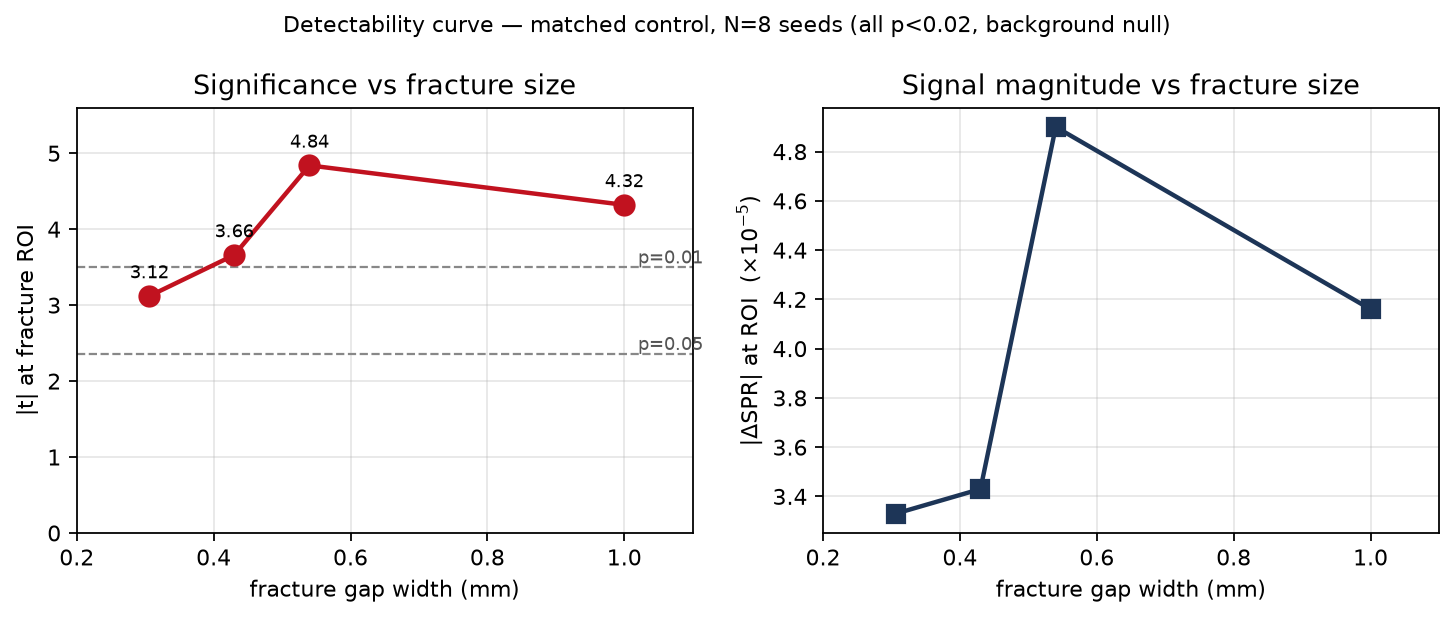
\includegraphics[width=0.99\linewidth]{fig/trend.png}
\end{center}
\vspace{-0.4ex}
{\small Signal rises with gap width from 0.306 to 0.54\,mm; $|t| = 3.1,\,3.7,\,4.8,\,4.3$.}
\end{block}

\begin{block}{4. Robustness \& Power (CL-1)}
\begin{itemize}
  \item Bootstrap 95\% CIs \textbf{exclude 0} for all sizes $\Rightarrow$ detections are real.
  \item Smallest fracture (0.306\,mm) is \textbf{borderline} (80\% reliability at $N{=}8$); $\sim$13 seeds reach $p<0.01$.
\end{itemize}
\vspace{-0.3ex}
\begin{center}
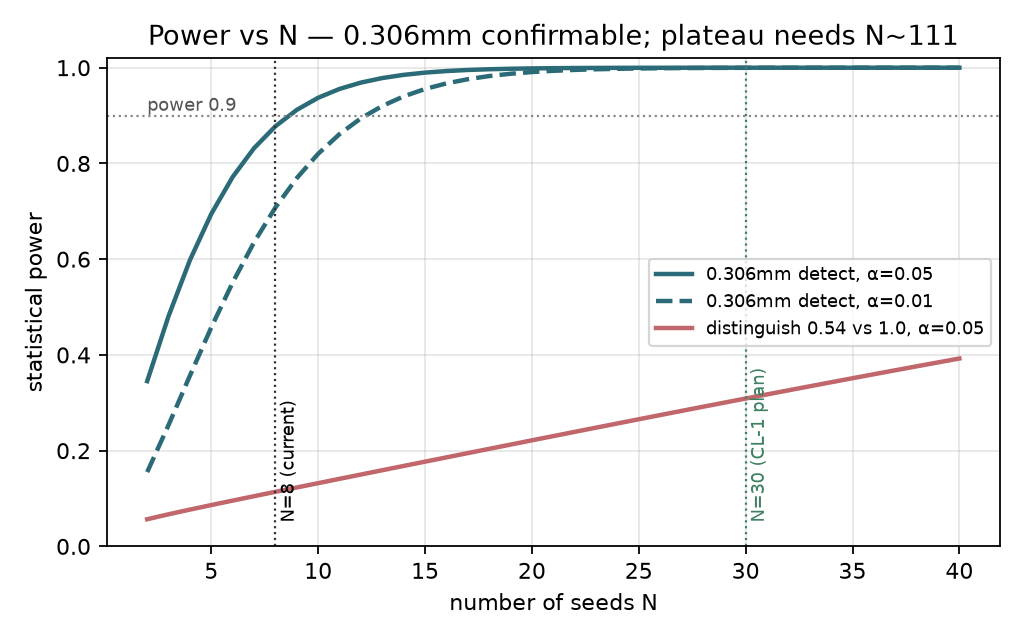
\includegraphics[width=0.82\linewidth]{fig_cl1/power.png}
\end{center}
\end{block}

\end{column}

% ================= RIGHT COLUMN =================
\begin{column}{.475\textwidth}

\begin{block}{5. Validity --- no false positives (CL-2)}
\begin{itemize}
  \item Control-vs-control false-positive rate $= 5.6\text{--}5.8\% \approx$ nominal 5\%.
  \item Sign-flip permutation confirms significance non-parametrically.
  \item Only $\sim$5\% of in-beam pixels significant (chance) $\Rightarrow$ \textbf{no global artifact}.
\end{itemize}
\vspace{-0.3ex}
\begin{center}
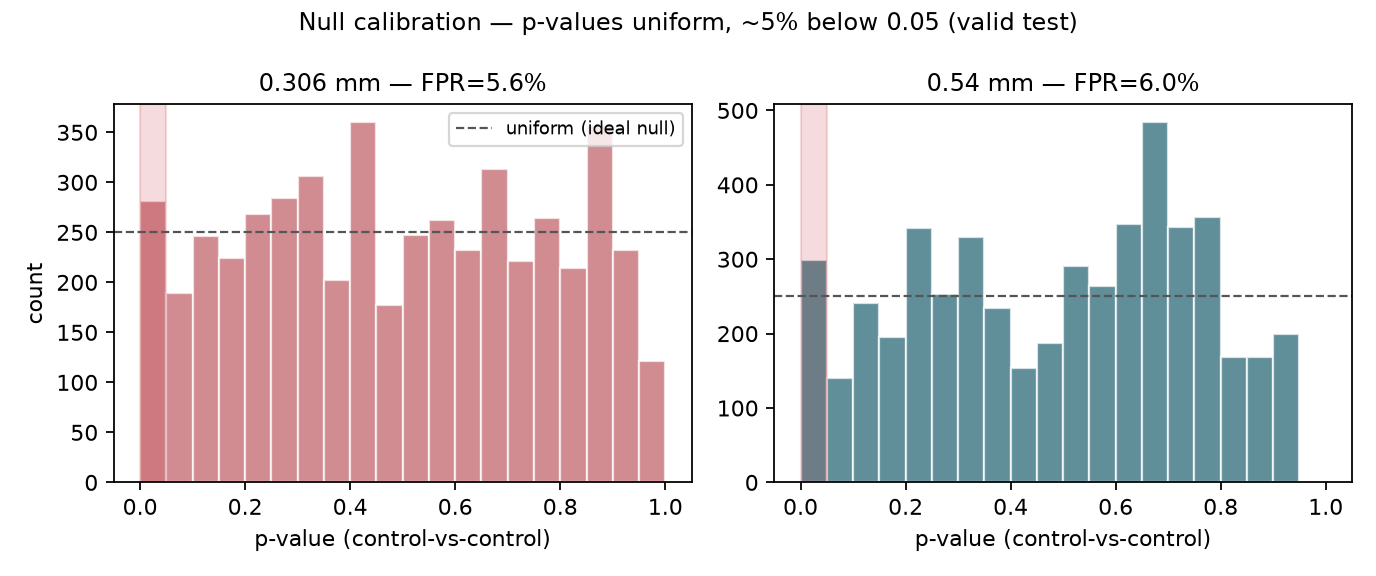
\includegraphics[width=0.99\linewidth]{fig_cl2/calib.png}
\end{center}
\end{block}

\begin{block}{6. Plateau resolution (CL-7)}
\begin{itemize}
  \item Signal rises 0.306$\to$0.54\,mm then \textbf{saturates} (0.54 $\approx$ 1.0, $p{=}0.73$).
  \item \textbf{Integrated} (spatial) signal saturates too $\Rightarrow$ saturation is \textbf{physical}, not an ROI artifact.
\end{itemize}
\vspace{-0.3ex}
\begin{center}
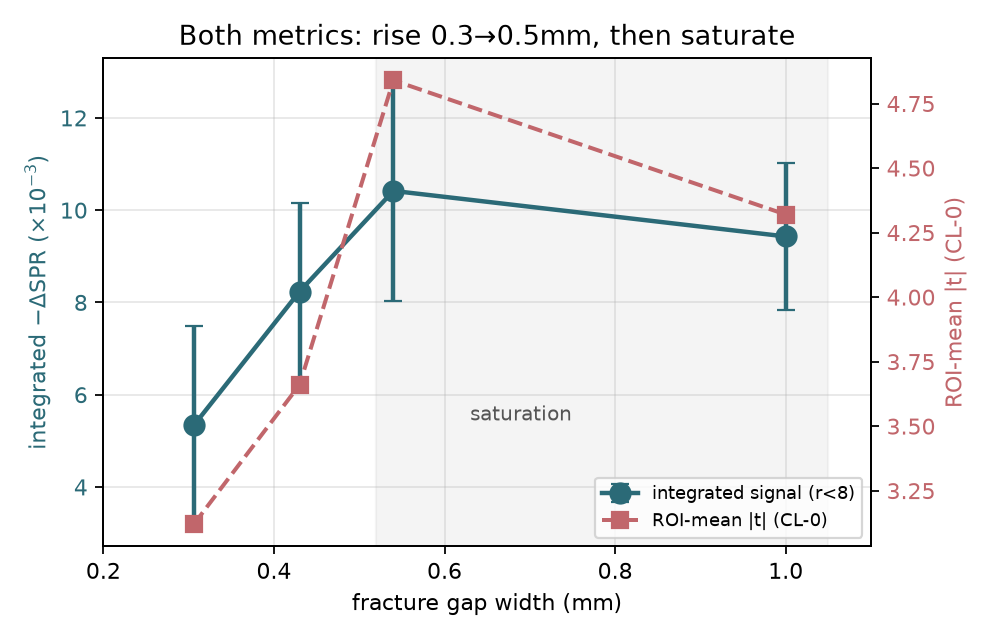
\includegraphics[width=0.92\linewidth]{fig_cl7/integrated.png}
\end{center}
\end{block}

\begin{block}{7. Mechanism tests --- in progress}
\begin{keybox}
\pend{CL-3 Energy dependence} (40--120\,keV): does the signal follow photoelectric/Compton physics? \quad\pend{[running]}\\[4pt]
\pend{CL-6 Beam-angle dependence}: is the signal maximal when the beam is tangential to the fracture plane (the clinical hallmark)? \quad\pend{[running]}\\[4pt]
{\small\color{muted} Results to be inserted in the final version; per-angle geometry pre-computed and queued.}
\end{keybox}
\end{block}

\begin{block}{8. Conclusions}
\begin{itemize}
  \item The SPR carries a \good{real, validated} fracture signature detectable to $\sim$0.3\,mm.
  \item The signal is \textbf{physically bounded}: excellent for \emph{detection}, saturating for \emph{width} $>0.5$\,mm.
  \item Energy- \& angle-dependence (pending) will complete the mechanistic proof for \textbf{Phase 1}.
\end{itemize}
\end{block}

\begin{block}{9. Phase-1 evidence pillars}
\centering
\renewcommand{\arraystretch}{1.25}
\begin{tabular}{cccccc}
\textbf{Detection} & \textbf{Robustness} & \textbf{Validity} & \textbf{Phys.\ bound} & \textbf{Energy} & \textbf{Geometry}\\
{\small CL-0} & {\small CL-1} & {\small CL-2} & {\small CL-7} & {\small CL-3} & {\small CL-6}\\[2pt]
\textcolor{ok}{\Large\checkmark} & \textcolor{ok}{\Large\checkmark} & \textcolor{ok}{\Large\checkmark} & \textcolor{ok}{\Large\checkmark} &
\textcolor{warn}{\small running} & \textcolor{warn}{\small running}\\
\end{tabular}
\end{block}

\end{column}
\end{columns}

\vspace{0.3ex}
\begin{center}
{\color{theme}\rule{\linewidth}{1.5pt}}\\[0.3ex]
{\small\color{muted} Repository: \texttt{intraprasart/GATE-Xray-pelvis-SPR} \quad$\bullet$\quad Method pillars: detection $\cdot$ robustness $\cdot$ validity $\cdot$ physical bound $\cdot$ (energy) $\cdot$ (geometry) \quad$\bullet$\quad contact: admin@baanwit.academy}
\end{center}

\end{frame}
\end{document}
